\documentclass[AMA,STIX1COL]{WileyNJD-v2}

\articletype{Article Type}%
\usepackage{graphicx}
\usepackage{caption}
\usepackage{subcaption}

\received{26 April 2016}
\revised{6 June 2016}
\accepted{6 June 2016}
\graphicspath{ {./images} }
\raggedbottom

\let\oldthebibliography\thebibliography
\let\endoldthebibliography\endthebibliography
\renewenvironment{thebibliography}[1]{
  \begin{oldthebibliography}{#1}
    \setlength{\itemsep}{0em}
    \setlength{\parskip}{0em}
}
{
  \end{oldthebibliography}
}

\begin{document}

\title{A Conversational Robot for promoting Social Distancing Awareness and Threat Monitoring along with an AI chatbot on Google Assistant\protect}

\author[1]{Niran N*}

\author[2]{Shreevallabha A}

\author[3]{T Prathyusha}

\author[4]{Manjunath R Kounte}

\authormark{Niran N \textsc{et al}}


\address{\orgdiv{School of Electronics and Communication Engineering}, \orgname{REVA Univeristy}, \orgaddress{\state{Bangalore}, \country{India}}}


\corres{*Niran N, School of Electronics and Communication Engineering, REVA Univeristy, Bangalore, India.
 \email{nirancodes@gmail.com, shreevallabhas@gmail.com, tpats2001@gmail.com, manjunath.kounte@gmail.com}}


\presentaddress{School of Electronics and Communication Engineering, REVA Univeristy, Bangalore - 560064, Karnataka, India}

\abstract[Summary]{The WHO has declared the the outbreak of covid-19 a pandemic. This unprecedented change is one of the first warnings to humanity to be ready for anything that may come in the future. Most of us in the community are unfamiliar with the sudden requirement of Social Distancing and maximum hygiene. It is critical to fully utilize today's technology in order to effectively address, manage, and live with these issues. We designed a conversational robot that uses Computer Vision to monitor the crowd flow and check if everyone is wearing masks, while primarily focusing on alerting people when Social Distancing is not followed and keeping them informed on the latest Pandemic information, A Chat Bot, integrated with Google Assistant, allowing anyone to get answers to all the questions about the pandemic while away from the community. We hope to use this system to combat the pandemic while preserving social distance.}

\keywords{Social Distancing, ChatBot, Pandemic Influenza, COVID-19, Computer Vision, NLP, Dialogflow, Google Assistant}

\maketitle

\jnlcitation{\cname{%
\author{Niran N}, 
\author{Shreevallabha A}, 
\author{T Prathyusha}, 
\author{Manjunath R Kounte}},
\ctitle{A Conversational Robot for promoting Social Distancing Awareness and Threat Monitoring along with an AI chatbot on Google Assistant}, \cjournal{Internet Technology Letters}, \cvol{}.}

\section{Introduction}\label{sec1}

% xLorem ipsum dolor sit amet, consectetuer adipiscing elit.\cite{Hirt1974}  

COVID-19, a coronavirus disease first identified in Wuhan, China, has rapidly spread across the globe and continues to spread with new strains. The WHO has declared it a pandemic. Globally, 64.35 million cases have been reported as of 4th December 2020. \cite{b1}. Even though the mortality rate has come down from 7.3\% (peak mortality observed on 25th Apr, 2020) to 2.3\% (on 4th Dec, 2020)\cite{b2}, the most concerning issue is that, the later phases of community spread has started in may parts of the world resulting in a huge increase in the number of cases reported. Social distancing has emerged as the most widely adopted strategy for its mitigation and control \cite{b3}.

Therefore, the second best option. other than staying put at homes, is to maintain self-hygiene, wear mask and social distancing measures \cite{b4}. Social distancing has proven to significantly reduce the risk of transmission. Massive public gatherings in schools, campuses, offices, halls and other public areas are being suppressed globally. We can't stay at home and lock down forever, so we need to take other precautions. \cite{b5}. This pandemic could benefit from the use of computer vision, a branch of artificial intelligence that analyzes and simulates visual data. It collects, stores, and transmits data to learn about the world. It combines mathematics, signal processing, and computer science. Computer vision is a great way to ensure social distancing.

\begin{figure}[t]
\centerline{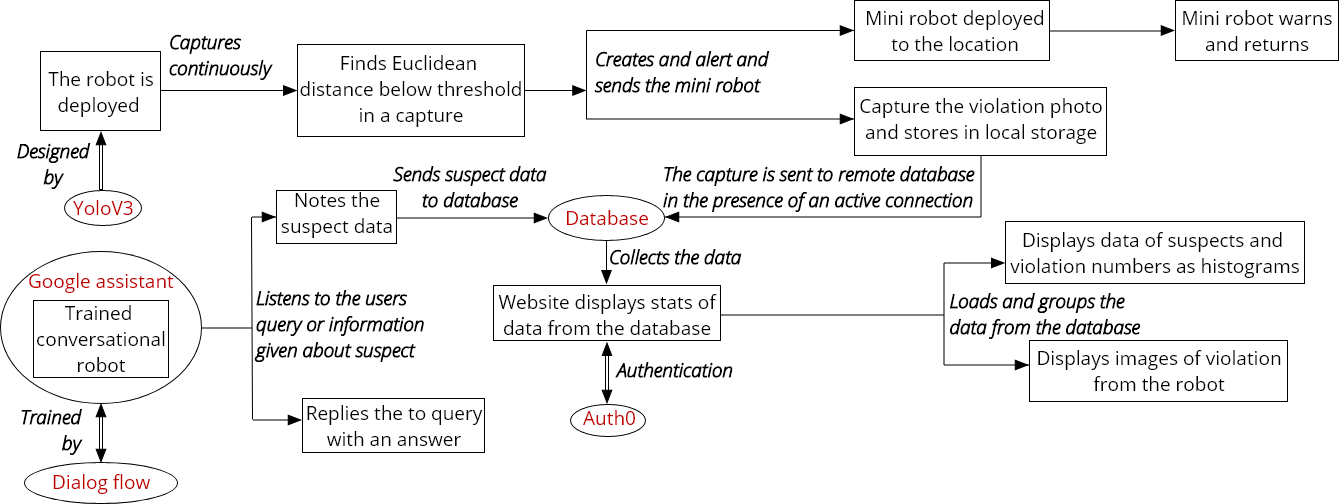
\includegraphics[width=1\textwidth]{obj_c.png}}
\caption{Objectives and workflow of the REDA System}
\label{fig1}
\end{figure}
%\begin{eqnarray}
%s(nT_{s}) &= &s(t)\times \sum\limits_{n=0}^{N-1} \delta (t-nT_{s}) \xleftrightarrow{\mathrm{DFT}}  S \left(\frac{m}{NT_{s}}\right) \nonumber\\
%&= &\frac{1}{N} \sum\limits_{n=0}^{N-1} \sum\limits_{k=-N/2}^{N/2-1} s_{k} e^{\mathrm{j}2\pi k\Delta fnT_{s}} e^{-j\frac{2\pi}{N}mn}
%\end{eqnarray}

\section{Theory behind Wang Reda}\label{sec2}

Humans tend to forget important points over time. The only way to be consistent is to have a reminder until it becomes a habit.
Long-term home quarantine is impossible. \cite{b6}.Even if COVID appears to have no end, people must work to survive. But this cannot be done without measures. \cite{b7}.

(a)  Should maintain distancing at least for another year

(b)  COVID-19 may spread again, if not taken care of.

(c)  Post corona life is expected to be different from normal life.

With regard to all these parameters, an apt system can be designed which can assist humans when in need and remind them about the protective measures that must be followed at all times \cite{b27} and warn them if the same is not followed. In this era of emerging technologies, an assistant who can interact with humans to provide COVID-19 related information easily through basic conversation and warn them automatically, when necessary is a must \cite{b8}.

\begin{figure}[t]
\centerline{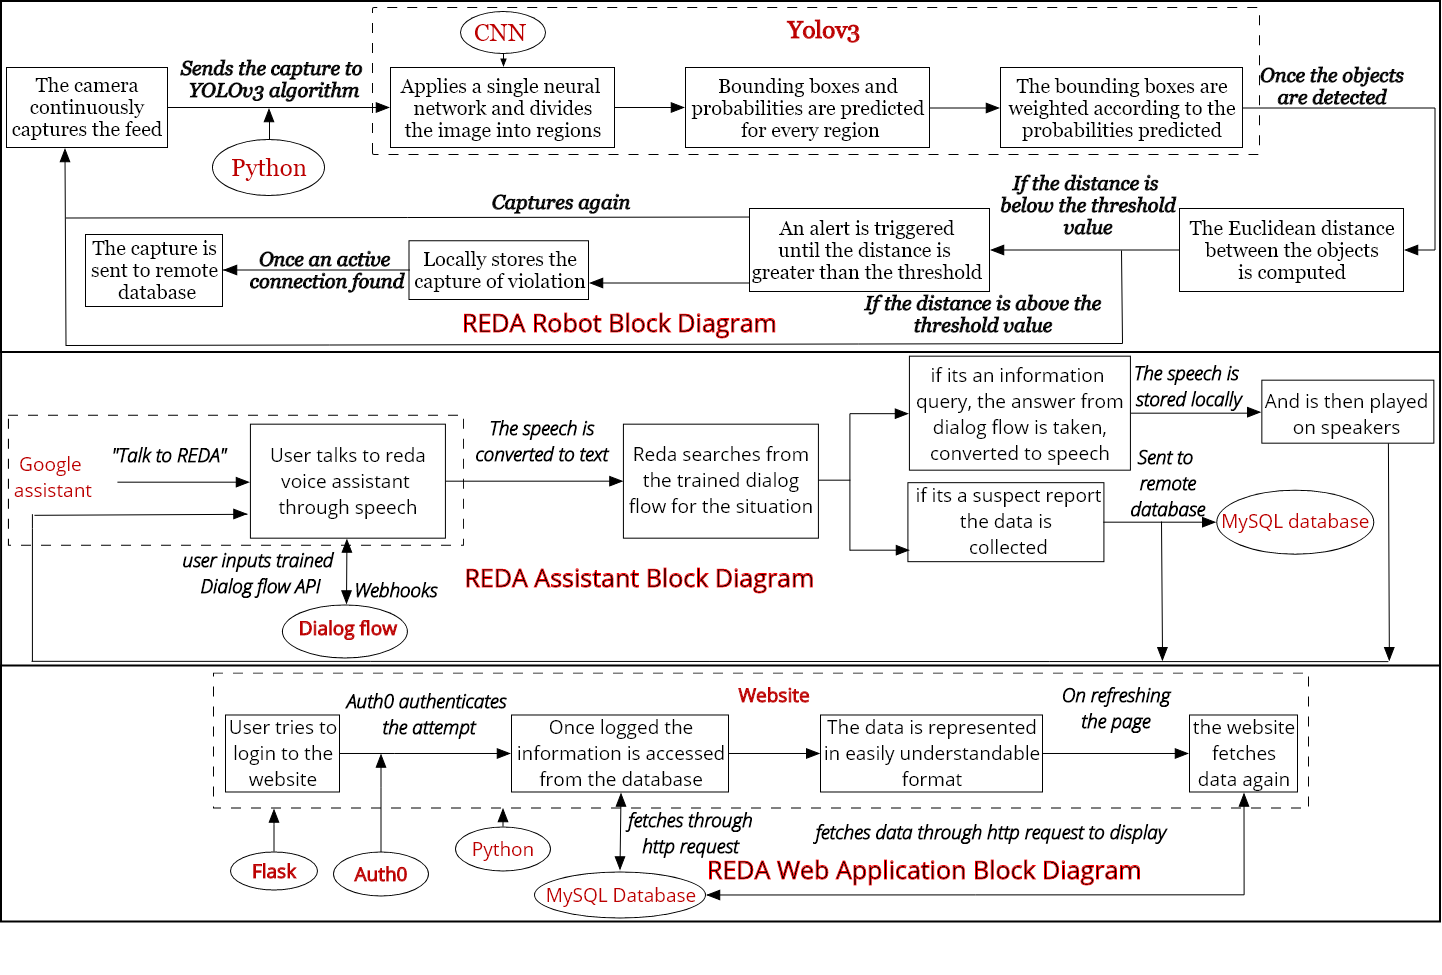
\includegraphics[width=1\textwidth]{reda3merge.png}}
\captionsetup{justification=centering}
\caption{(a) Process flow schema for working of the proposed  REDA Robot (b)Process flow schema for working of REDA Virtual Assistant (c)Process flow schema for working of REDA's Web-App}
\label{fig2}
\end{figure}

%\begin{figure}[t]
%\centerline{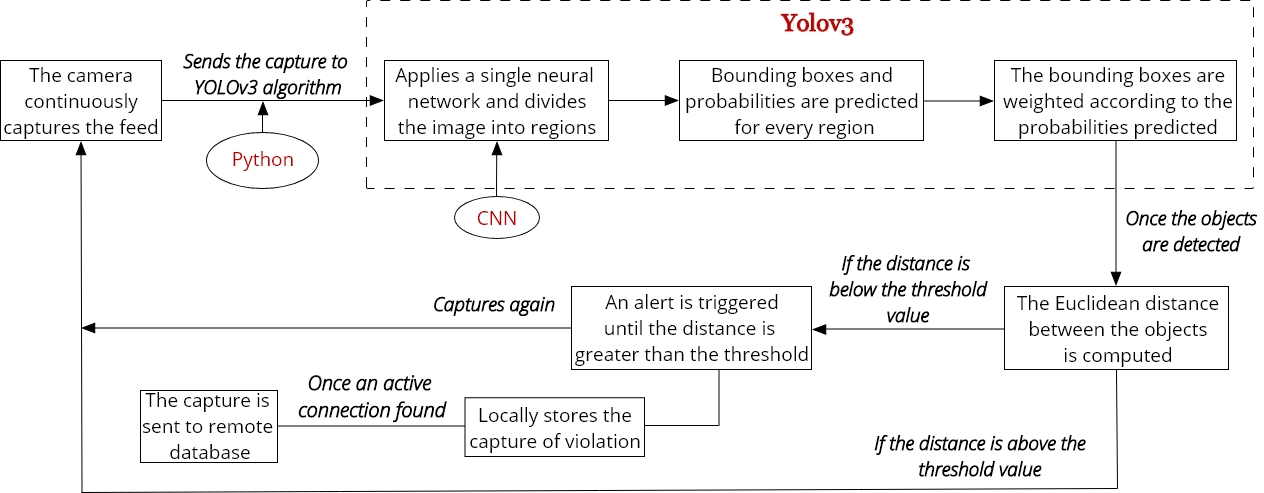
\includegraphics[width=1\textwidth]{Redarob.jpg}}
%\caption{(a) Process flow schema for working of the proposed  REDA Robot (b)Process flow schema for working of REDA Virtual Assistant (c)}
%\label{fig2}
%\end{figure}

We used YOLO’s object detection algorithm to find the objects in the scenery. Compared to other projects the object detection is very rigid and accurate. The robot is self sufficient to answer any typical questions related to the pandemic and give health care tips. In recent times, there have been many solutions coming up to face the challenge of social distancing. Devices like wristbands, shoulder bands or small handy devices to carry on in pockets are very effective \cite{b9} but they have their drawbacks. Ensuring the goal being fulfilled is very important and urgent. Hence, we cannot spend a lot of time in manufacturing billions of units to meet the demand of the population \cite{b10}. One Wang Reda can replace many such devices reducing the time and effort to manufacture units. As the robot is capable of handling large crowds by itself, an organization can get the unit installed at their work space to monitor all their employees.

The robot is enabled to communicate with IoT devices \cite{b26}. The robot reports to the server regarding every event where social distancing is violated. Thus the organization can keep track of the reports and take necessary actions. The robot is capable of receiving user complaints. People can report any person they suspect of having COVID-19 or showing any symptoms to the robot. The data will be captured and securely stored, allowing administrators to trace contacts and take necessary steps.

%\begin{figure}[t]
%\centerline{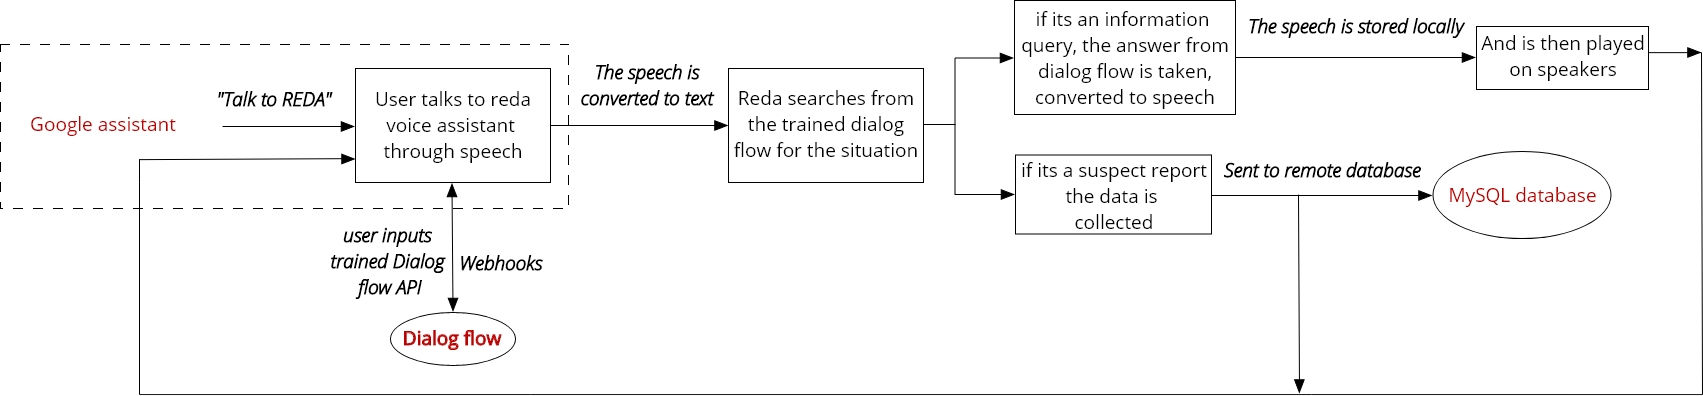
\includegraphics[width=1\textwidth]{Redava.jpg}}
%\caption{Process flow schema for working of REDA Virtual Assistant}
%\label{fig3}
%\end{figure}


\section{Objectives and Deliverables of the System}  \label{boba} 

The scope that we are trying to cover through this robot is vast. Not only can the functions be upgraded over time, the same script can be utilized for multiple scenarios where there's a need for a conversational robot.  Below are the few points which we believe would be a major factor when it comes to the scalability and flexibility of this project.

\textbf {Diversity} - Unlike other bots, Wang Reda can communicate through multiple platform, promoting Diversity and giving out access to everyone easily, at virtually no cost. 

\textbf {Working} - Reda can be controlled wirelessly, thus promoting a remote accessible environment, which is essential for today’s world. The script can be run and updated through cloud and the dashboard can be used to monitor the status

\textbf {Tech and Wealth} - The primary motive of building Reda was to prevent the COVID-19 virus from spreading via person-to person. Millions of people have died \cite{b11}, and the only way to prevent more deaths until a permanent cure is to promote social distancing and hygiene. 

 \textbf {Creating Awareness} - Reda’s multi platform accessibility and Conversational UI makes it possible to bring awareness about the current situation to the user. Frequent updates, social distancing violation detection and warning, suspect alert and emergency alerts are some of the functionalities. The new dashboard feature added to the same via our web app allows the user to seamlessly check current information of the pandemic and check the suspect reports and other gallery based information.


\subsection{Main Objectives of developing Reda}

\quad(a) Create a Conversational Robot that can speak with people using Natural Language Processing (NLP). It can also take in inputs from people with respect to any suspects that can be found in the vicinity.

(b) Create a Mini Robot that can travel to that location and warn people about Social Distancing. If the main robot detects any violation from any of the cameras, the mini robot can go warn people to maintain social distance.

(c) Create a web-app for the robot that allows users to see all collected data about physical distance violations.

(d) Training the Robot to use Dialog Flow to answer queries. The AI chat bot integrates with Google Assistant so users can easily get information or report something. REDA can converse with people in a natural human tone (doesn't use a robotic voice - hence friendlier).

(e) A robot that can warn people when Social Distancing is not maintained - Using open CV and implementing YOLO to train a program to detect if Social Distancing is being followed. 

(f) The WebApp contains a histogram dashboard showing the daily count of violations, details entered by the chatbot, and a gallery of photographs acquired by the robot.

(g) The capabilities and the features of the bot are not limited to Hardware! The chat assistant part of the system can be accessed using Google Assistant.


%\begin{itemize}
%\item Create a Conversational Robot that can speak with people using Natural Language Processing (NLP). 

%\item Create a Mini Robot which can travel to that designated place and read out a warning to them to follow Social Distancing

%\item Create a web-app for the robot that allows users to see all collected data about physical distance violations.

%\item Training the Robot to use Dialog Flow to answer queries. The AI chat bot integrates with Google Assistant so users can easily get information or report something.

%\item A robot that can warn people when Social Distancing is not maintained - Using open CV and implementing YOLO to train a program to detect if Social Distancing is being followed. 

%\item The WebApp contains a histogram dashboard showing the daily count of violations, details entered by the chatbot, and a gallery of photographs acquired by the robot.
%\end{itemize}

\subsection{Key Deliverables of our Robot}


\quad(a) An autonomous conversational robot pre-programmed to help humans with their queries.

(b) Almost any query related to the COVID pandemic can be conversed.

(c) The robot can detect humans and see whether social distancing is being followed.

(d) Robots can take in feedback from humans to improve environmental conditions.

(e) Humans can report a suspect and the same will be forwarded to the authorities asap.

(f) The Robot can be summoned through Google Assistant on their phones when it is not in their vicinity. The AI based conversational bot can provide essential information about the current COVID status. The suspect report can also be conducted.

(g) All the data recorded by both the robot and the chat bot are sent to the Web-App through a remote database and updated timely.

\section{Design, Development and Implementation of System}

Our aim is to create a robot that can navigate, respond to user queries and monitor physical distance as the primary goal. When it comes to working with AI and Robot-based initiatives, Raspberry Pi comes in handy \cite{b12}. Below are a some of the main technologies that we are utilizing to build and run Wang Reda. A brief description of the technology along with how we are utilizing has been discussed below.

%\begin{figure}[t]
%\centerline{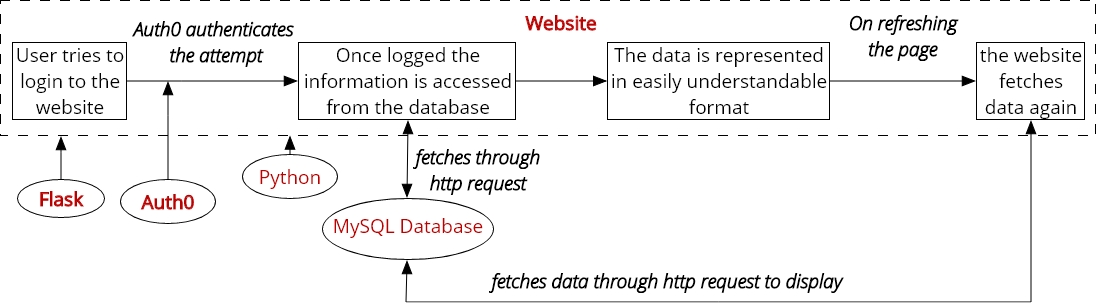
\includegraphics[width=1\textwidth]{Redaweb.jpg}}
%\caption{Process flow schema for working of REDA's Web-App}
%\label{fig4}
%\end{figure}



%\textbf {YOLO:}YOLO is a real-time object detection algorithm. The algorithm applies the complete image to a single neural network, then splits the image into regions and forecasts bounding boxes and probabilities for each region. If the distance is less than the threshold value, the user is alerted to comply with rules of social distancing. \cite{b13}.

%\textbf{Dialog Flow:}
%Dialog Flow is a natural language understanding platform used to design and integrate a conversational user interface into mobile apps, web applications, devices, bots, interactive voice response systems, and so on. The same can be noted in Google Assistant as mentioned earlier, wherein you can talk to REDA on your phone! \cite{b14}.

%\textbf{Flask:}
%Flask is an extremely light-weight web framework written in Python \cite{b15}. The flask-sqlalchemy package helps in connecting a database to a Flask application. Once the data from the database is obtained it is updated on the Web-App accordingly for easy analysis. We have used flask with python as the programming language to establish a connection between the Web App and the database.

The robot captures continuously and the camera feed to sent to the program which applies YOLO detection to the image frames. It applies a single neural network to the full image. This network divides the image into regions and predicts bounding boxes and probabilities for each region. These bounding boxes are weighted by the predicted probabilities. Once the objects in the image are recognized, euclidean distance \cite{b17} is computed. If the euclidean distance is less than the threshold (which is tuned), an alert is triggered until the social distancing is maintained.
This captures and stores the image in local storage. The images are uploaded to the server storage when there is an active connection and the record is made available in the database along with the necessary details such as date, time stamp and location.
The Web-App is served using a flask application. An administrator can authorize the Web-App and can view the reports and the statistical view of the breaches made.

While one part of the program focuses on image recognition, the other part ensures that the robot is able to communicate in real time with the user. This section enables the robot to answer any of the questions that are given to it. The robot can answer the general questions asked about the campus/office, the location where it was installed, FAQs, tips on how to avoid COVID-19, current statistics and many more \cite{b18}. The robot uses a user inputs-trained dialog flow API. Once the dialog flow has been trained, the user queries can be responded to with ease. Thus, all the possible questions and answers have to be fully trained in the dialog flow. Again, DialogFlow makes it possible to provide an answer for the recognized text and reply accordingly. Using gTTS API \cite{b19}, the obtained text is then converted from text to speech. After this response is generated in the form of speech, the result obtained is returned to the user. The speech is therefore saved in the local storage and is played by speakers.

For some queries, the bot may also take in the user's inputs if required. The robot is capable of receiving reports provided by citizens about suspects. Reports are inserted into the MySQL database. Supposing that there is an incident or a suspicious person that you want to inform about, that can be done through the application anonymously. Using an  API, user input is given through speech, then converted to text. The text obtained is sent to the dialog flow to get the result, which is the response to the text of the query. The data obtained during the dialog flow is then sent via a webhook to our storage database and the information collected can be viewed by the authorities as soon as they authenticate themselves on the web portal. The administrator can see the reports and take the necessary measures. A pre-defined response is given as a response to the user.

The above mentioned section of conversation can also be conducted using Google Assistant available on any phone. This way, the robot becomes truly flexible, allowing the user to enquire as and when needed, even if they are not around the nearest robot to converse. It also makes them stay updated to the latest information given by the university/office where this is placed with ease. If any COVID suspect is reported in the campus, he/she can be bought to the notice of the authorities, the same can be carried out with Google Assistant on which Reda has been enabled. As of now, Reda has been rolled out on Beta and not available for the public. One can access Reda by opting in for the same through the Web-App.

\begin{figure}
\centerline{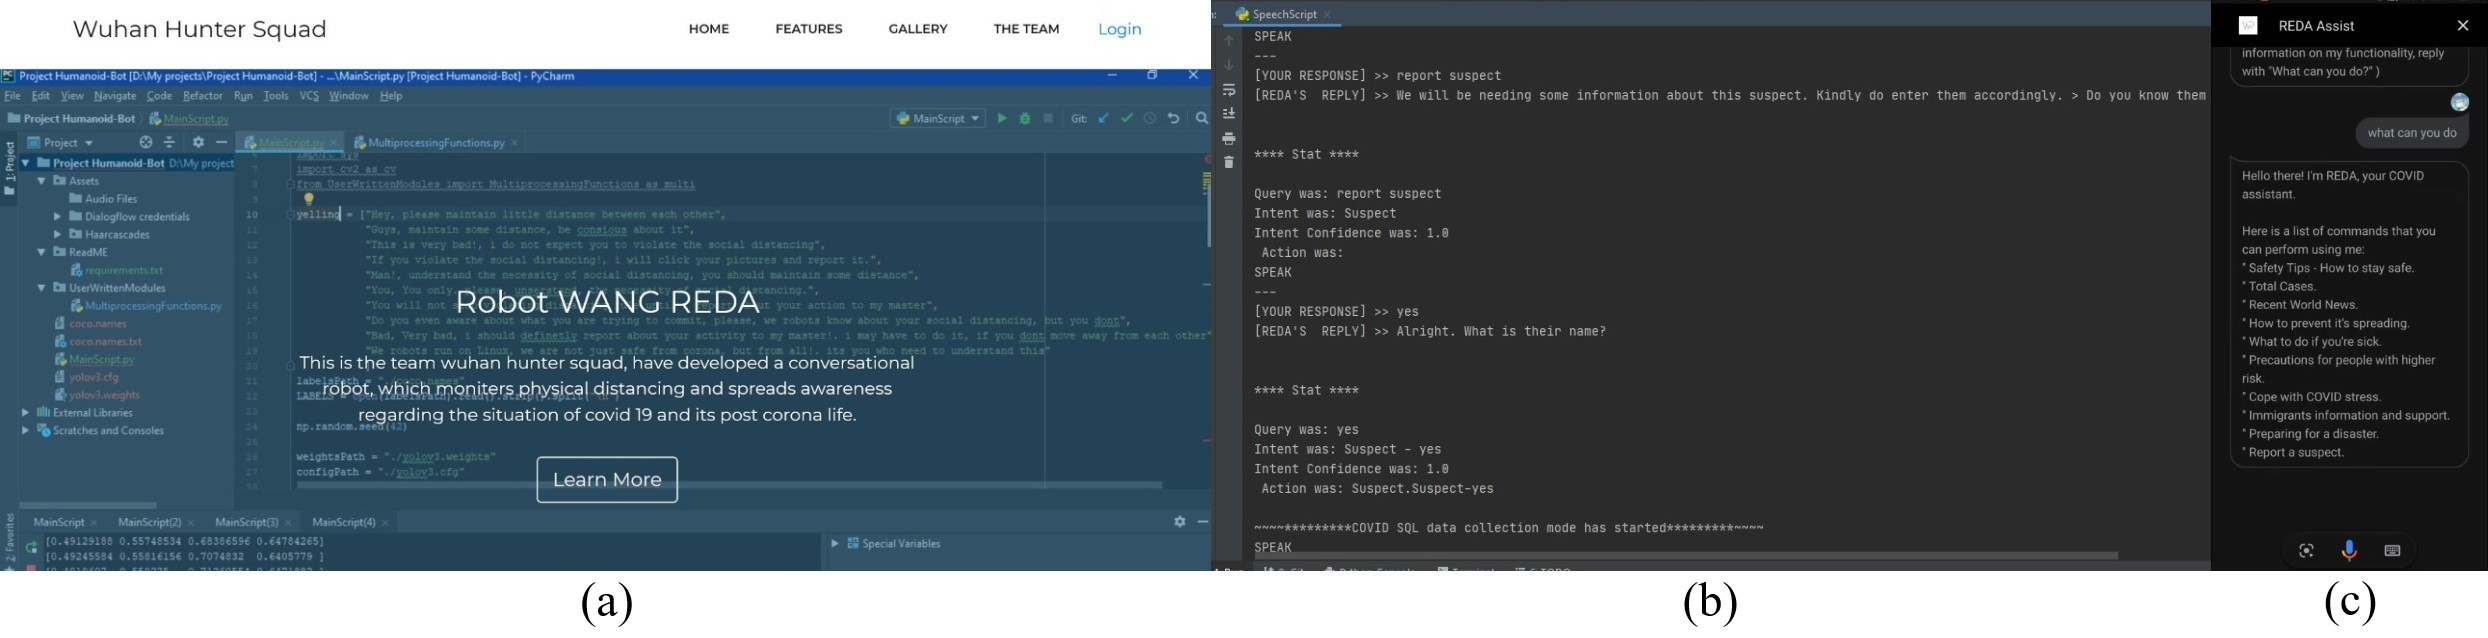
\includegraphics[width=1\textwidth]{webf.jpeg}}
\captionsetup{justification=centering}
\caption{(a) Welcome Screen of REDA's Web-App  (b) Reporting of Suspects/Cases to the bot through Voice \\(c) Accessing REDA through Google Assistant 
\label{fig5}}
\end{figure}
\begin{figure}
\centerline{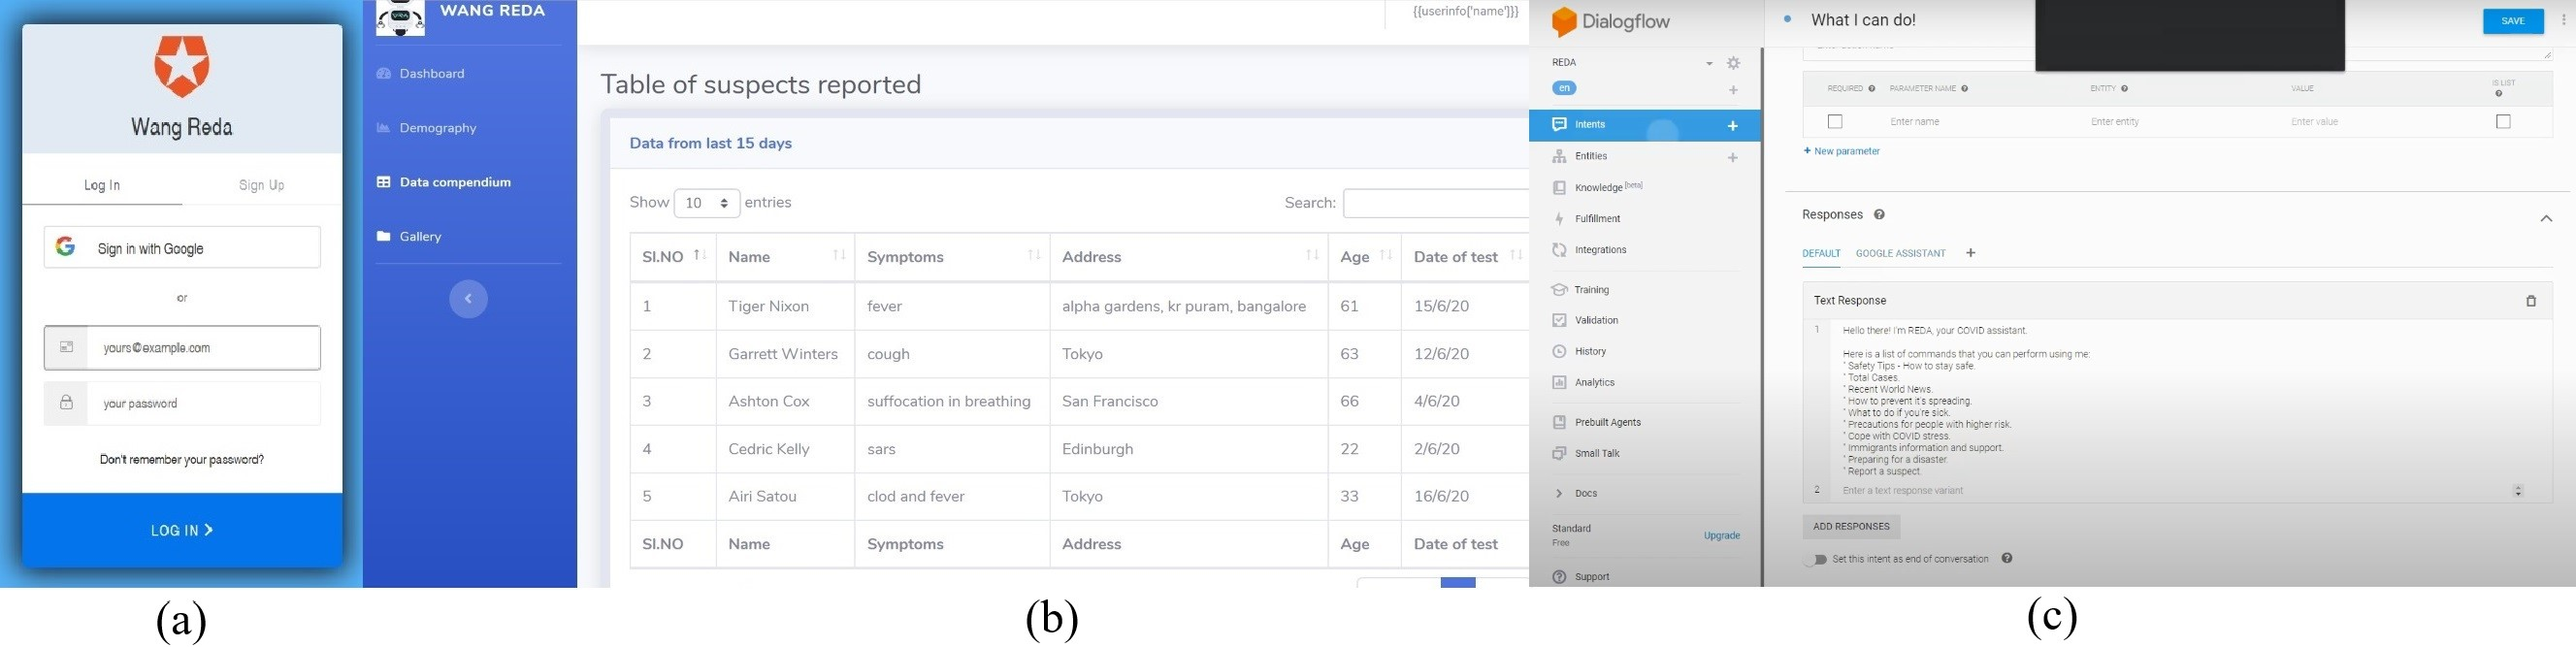
\includegraphics[width=1\textwidth]{webd.jpeg}}
\captionsetup{justification=centering}
\caption{(a) Provision for admin to login and access dashboard (b) List of suspects/confirmed cases in the community \\(c) Glimpse of Program Schema in DialogFlow
\label{fig8}}
\end{figure}
\begin{figure}
\centerline{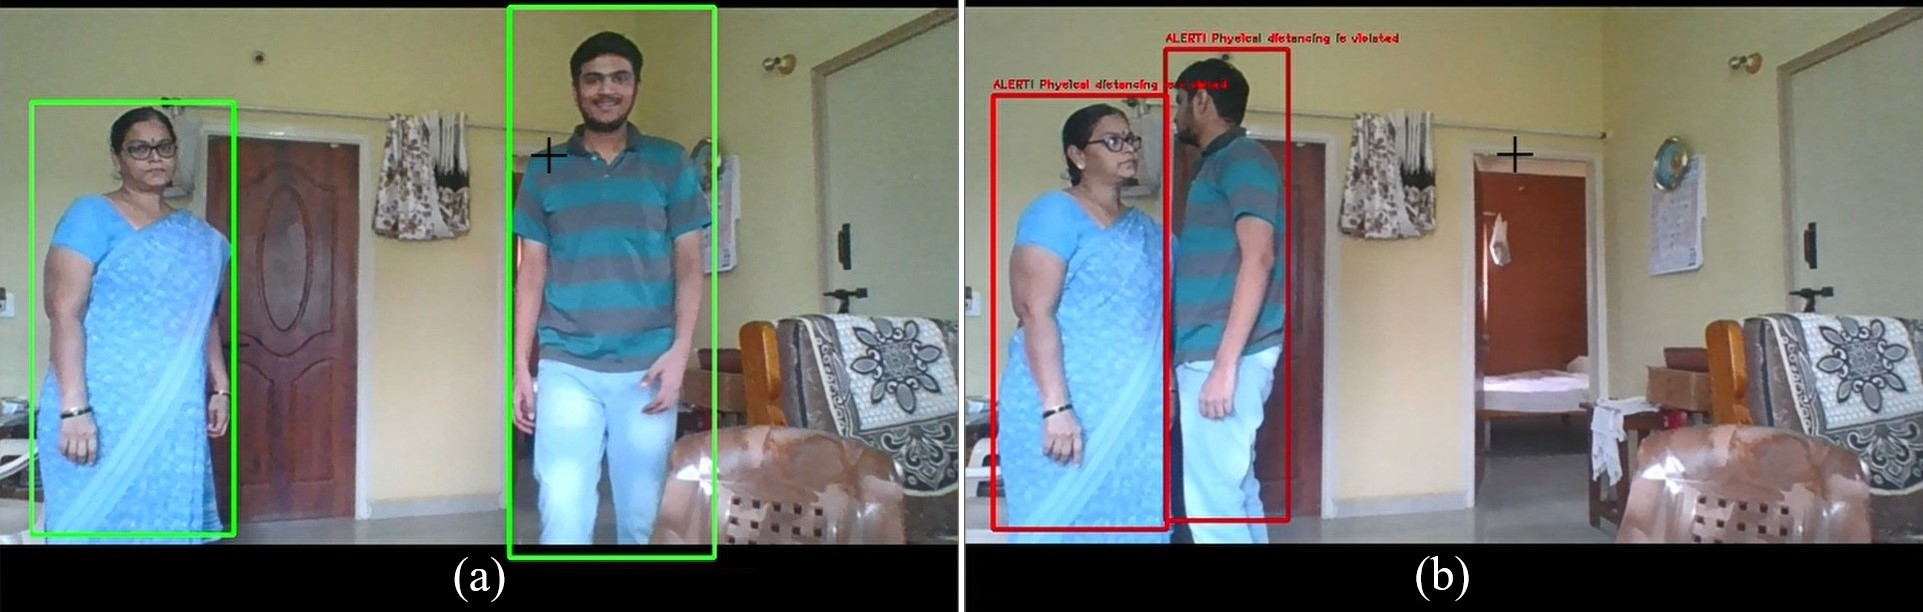
\includegraphics[width=1\textwidth]{sdok.jpeg}}
\captionsetup{justification=centering}
\caption{(a) AI detects that Social Distancing is being followed \\(b) AI detects that Social Distancing not being followed - Program detects \& sends out a warning to that Civilian
\label{fig8}}
\end{figure}

\section{Results and Discussion}

After months of research, prototyping and programming, we were able to obtain a fruitful result. The operations mentioned in section \ref{boba} are working successfully as they should have. The Web-App is hosted at https://redais.online where the authenticated users can login and manage the bot they have the control for. The Web-App also contains a simple manual of the robot, its features, a glimpse on the product through the gallery and the team behind it. We have also introduced a miniature version of our chat bot on the Web-App through which basic questions and queries can be conversed. We believe that this robot that was developed has loads of potential and can be used for other situations, not just the current pandemic. Some of the images that were taken during the development and of the working prototype are attached. 

%\begin{figure}[!h]
%\centerline{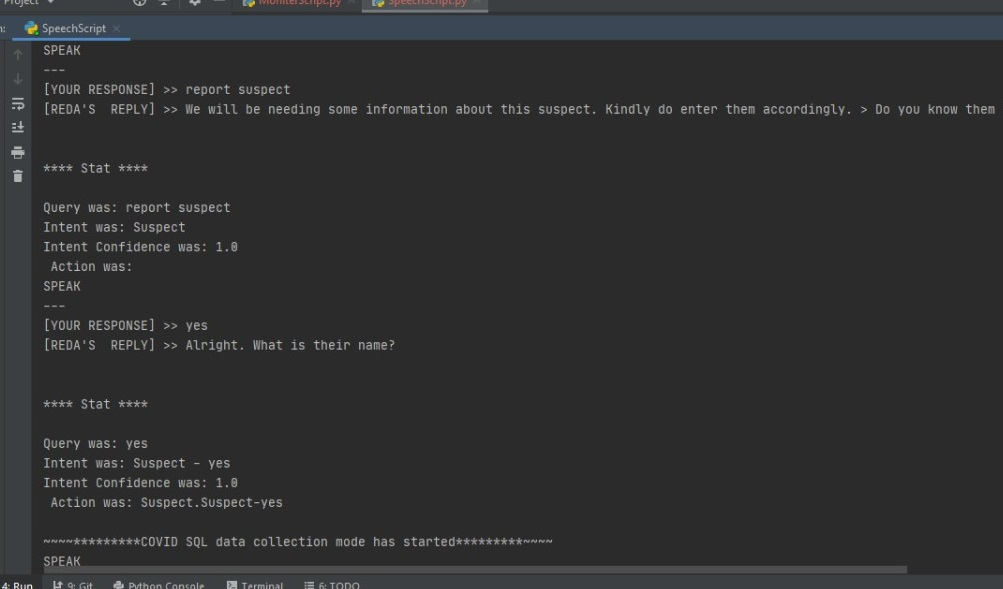
\includegraphics[width=400pt]{sus.jpeg}}
%\caption{Reporting of Suspects/Cases to the bot through Voice
%\label{fig6}}
%\end{figure}
 
%\begin{figure}[!h]
%\centerline{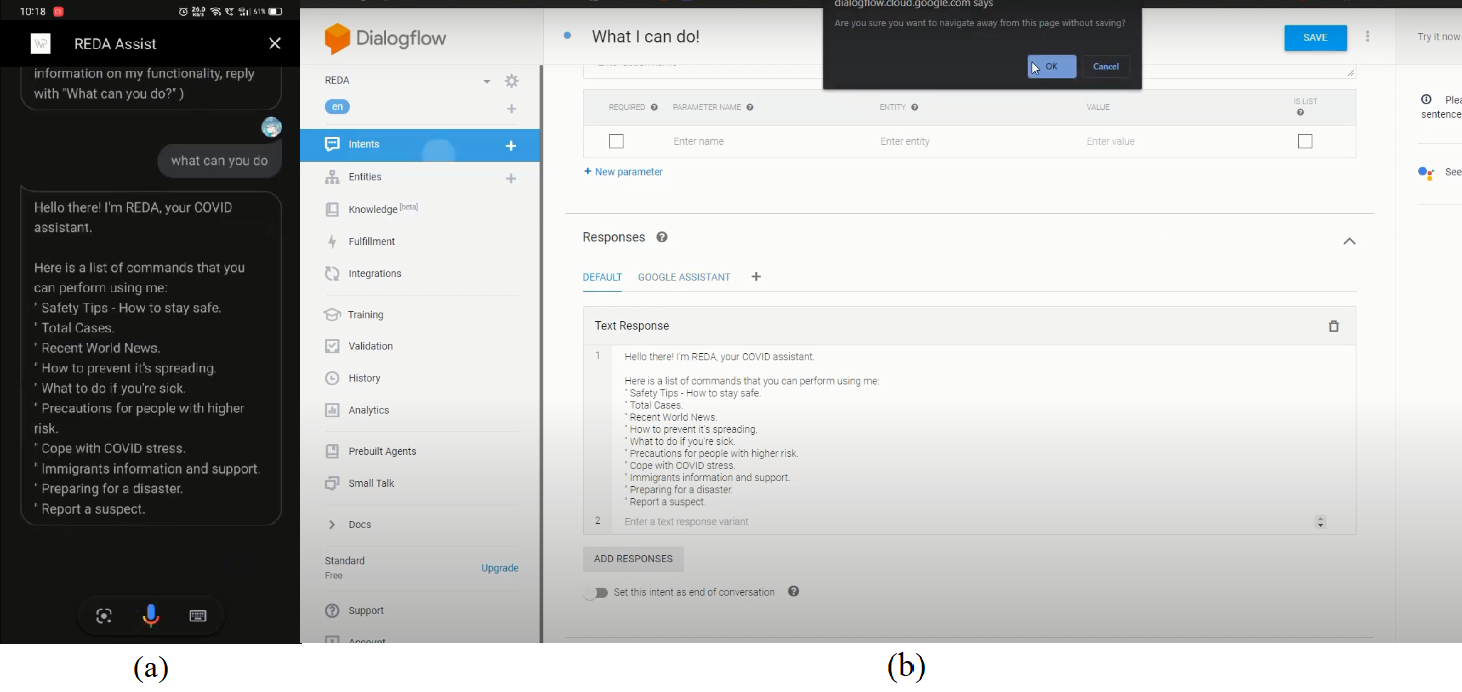
\includegraphics[width=480pt]{dfa.png}}
%\captionsetup{justification=centering}
%\caption{(a) Accessing REDA through Google Assistant \\(b) Glimpse of Program Schema in DialogFlow
%\label{fig7}}
%\end{figure}

%\textbf{Prevent 2nd peaking of COVID once the pandemic affected rate decreases -}
%It is very essential and important to maintain social distancing even after the cases number drops. This is important because if humans become casual and forget the severity of the virus, the disease would spread rapidly and cause a second wave of death \cite{b20} \cite{b21}. (Ref: The Case of Smallpox in Europe where lack of hygiene caused mass mortality \cite{b22}) 

%\textbf{Remind people to maintain social distancing - }
%People tend to forget social distancing, especially when with friends and pals. We are not used to maintaining such distances for a long time and might forget about it unintentionally \cite{b23}. At such times, the robot is of really good use to remind people about the same. The mini robot that can communicate with the main robot can go and warn people to maintain social distancing if the main robot detects any violation from any of the cameras. 

%\textbf{Assist people with tips and information: Carry out conversation -}
%REDA can converse with people in a natural human tone (doesn’t use a robotic voice - hence friendlier) and can respond to almost any of their queries with respect to COVID (We pre-trained it to adapt to human language; uses Dialog Flow).
%It can also take in inputs from people with respect to any suspects that can be found in the vicinity. Such inputs are forwarded to the respective authorities so that further investigation and possible quarantine of that person could be conducted for the benefit of the others \cite{b24}. 

%\textbf{Robot and beyond! -}
%The capabilities and the features of the bot are not limited to Hardware!
%Any person who has an Android phone (v 7.0 and above) / iPhone 5S and above can use Google Assistant \cite{b25} to converse with REDA. By telling “Talk to REDA Assist”, they can speak to the robot and obtain helpful information wherever they are. This would be very useful in Huge campuses and offices where users cannot contact REDA often when they have a query.

%\section{Assumptions and Limitations}

%\subsection {Assumptions made while Development}
%There are some assumptions that were taken into consideration while the robot was being developed. Satisfying these assumptions is essential to ensure the proper functioning of the robot, until further development on these sections could be done.

%\begin{itemize}
%\item The organization has decent accessible Wi-Fi. The program cannot work without an active internet connection.
%\item The organization must be able to bear the robot’s cost.
%\item Since the mini robot is movable (via wheels), the robot might be prone to damage if humans mishandle it (The robot has Obstacle Avoidance feature built-in, but it’s always better if %humans are aware). Hence, proper guidelines must be issued when in use. 
%\item Initial calibration necessary for accurate Social distancing measurements. 
%\item Language for conversation - only the standardized version of  English can be used
%\item Google Assistant requirements - Android 7 and above.
%\item Special designated outdoor environment for the robot is required, preferably with proper paved tracks/roads. The same must be protected from Natural events like rain. (Robot’s %current prototype is NOT waterproof)
%\end{itemize}
\section {Conclusion}

With the pandemic, we have learnt the value and importance of self-hygiene and social distancing.. We all know that life will not be normal for a few more years, so we must take all possible precautions to stop the spread of this deadly disease. WangReda was created to help us all in these difficult times. It uses modern technology to monitor and raise awareness about social distancing in crowds. It is a robot with computer vision to check if people are wearing masks, maintaining social distancing and warn them if violated. The Google Assistant-powered chatbot can be used on any smartphone to answer questions about the pandemic and collect suspect data. To make contact tracing easier, it stores and displays all required information on the Web-application for authorized users.

WangReda opens new doors to not only monitor social distance but also to solve many real-world issues. WangReda's technology is vast and can do wonders when worked on with focus. We believe Reda has a lot more potential and will soon have even more features to help countless people.

%\nocite{*}% Show all bib entries - both cited and uncited; comment this line to view only cited bib entries;
\bibliography{wileyNJD-AMA}

\end{document}
